\chapter{Results and Discussion}
In the previous chapters, we have laid the theoretical and methodological foundations of our investigation:  
from the gravitational wave theory, to the astrophysical context of white dwarfs and their host galaxies, the principles of gravitational wave detection, and finally the construction of the simulated populations used in this work.  
In this chapter, we turn to the quantitative generation of the corresponding gravitational wave signal.  
We begin by completing the list of galaxies that we use as a reference for the simulations, by taking into account for the incomplete entries of the GWGC and the galaxies obscured by the Zone Of Avoidance.
Afterwards, we generate the fixed populations that are used to simulate all the galaxies, by choosing the corresponding metallicity values based on the range covered by the galaxies in the final catalog.
After discussing LISA's frequency resolution, and understanding how to take it into account, we are able to apply the computational pipeline described in the previous chapter to our final galaxy catalog, extracting the gravitational wave signal from the simulated populations of binary white dwarfs.  
The resulting spectra are then compared to the LISA sensitivity curve to verify the detectability of an extragalactic background.  
Finally, we discuss the frequency distribution and amplitude characteristics of the simulated signals, as well as the physical reasons underlying our results, and their implications for future space-based gravitational wave detectors.


\section{Preparations}
Before computing the total extragalactic DWDs gravitational foreground, we must ensure that our list of galaxies is truly representative of the total population of DWDs in the local universe. 
This means we must consider that the final catalog that we use to compute the signal is incomplete, analysing both the internal and the external causes of lack of galaxies.
Only then, we can group the final galaxies in terms of metallicity, and generate the fixed populations that will be used to reproduce the DWDs hosted in them.
These two steps will lay the ground for the gravitational signal generation and processing.

\subsection{Missing galaxies}
The GWGC is far from being a complete list of the galaxies in the local Universe, and there are two main factors contributing to this: observational limitations due to the Zone of Avoidance (ZOA) and limitations of the information that the catalog presents.

\subsubsection{GWGC incompleteness and non-galactic objects}
The entries of the GWGC represent a source of incompleteness themselves. 
Not all the objects listed in the GWGC are suitable for our purposes:
in addition to galaxies, the catalog also includes globular clusters, which can be identified through their T-type values; 
moreover, not all galaxies in the catalog contain all the information required to perform the procedures described in the previous sections.
To construct a working sample, we applied a series of masks to clean the catalog:
\begin{itemize}
    \item Only keep entries classified as galaxies; 
    \item Require that the distance, T-type, and absolute blue magnitude are provided; 
\end{itemize}
After this selection, the sample we are left with scaled down in size, from the original $53,255$ entries to $20,246$ galaxies suitable for population synthesis.

\subsubsection{Zone of avoidance}
Since the GWGC is an observation-based catalog derived from optical surveys, we must account for the Zone of Avoidance, the region of the sky obscured by the Milky Way’s interstellar dust and stellar crowding, which impedes the detection of background galaxies.
The extent of the ZOA depends on the wavelength of observation: infrared surveys penetrate deeper through the dust, while optical surveys, like those used for GWGC (the reported magnitude for these galaxies is in the B-band), are more strongly affected. 
In the optical band, the ZOA is expected to cover about $\sim25\%$ of the sky, as reported in~\cite{Kraan-Korteweg}.
For this work, we estimated the ZOA directly from the spatial distribution of galaxies in GWGC, by plotting their positions in Galactic coordinates, and highlighting the empty regions of the sky. 
This way, the ZOA appears clearly as a horizontal band centered around the Galactic plane (see \textbf{Figure~\ref{fig: ZOA in galactic coordinates}}).
\begin{figure}
    \begin{center}
        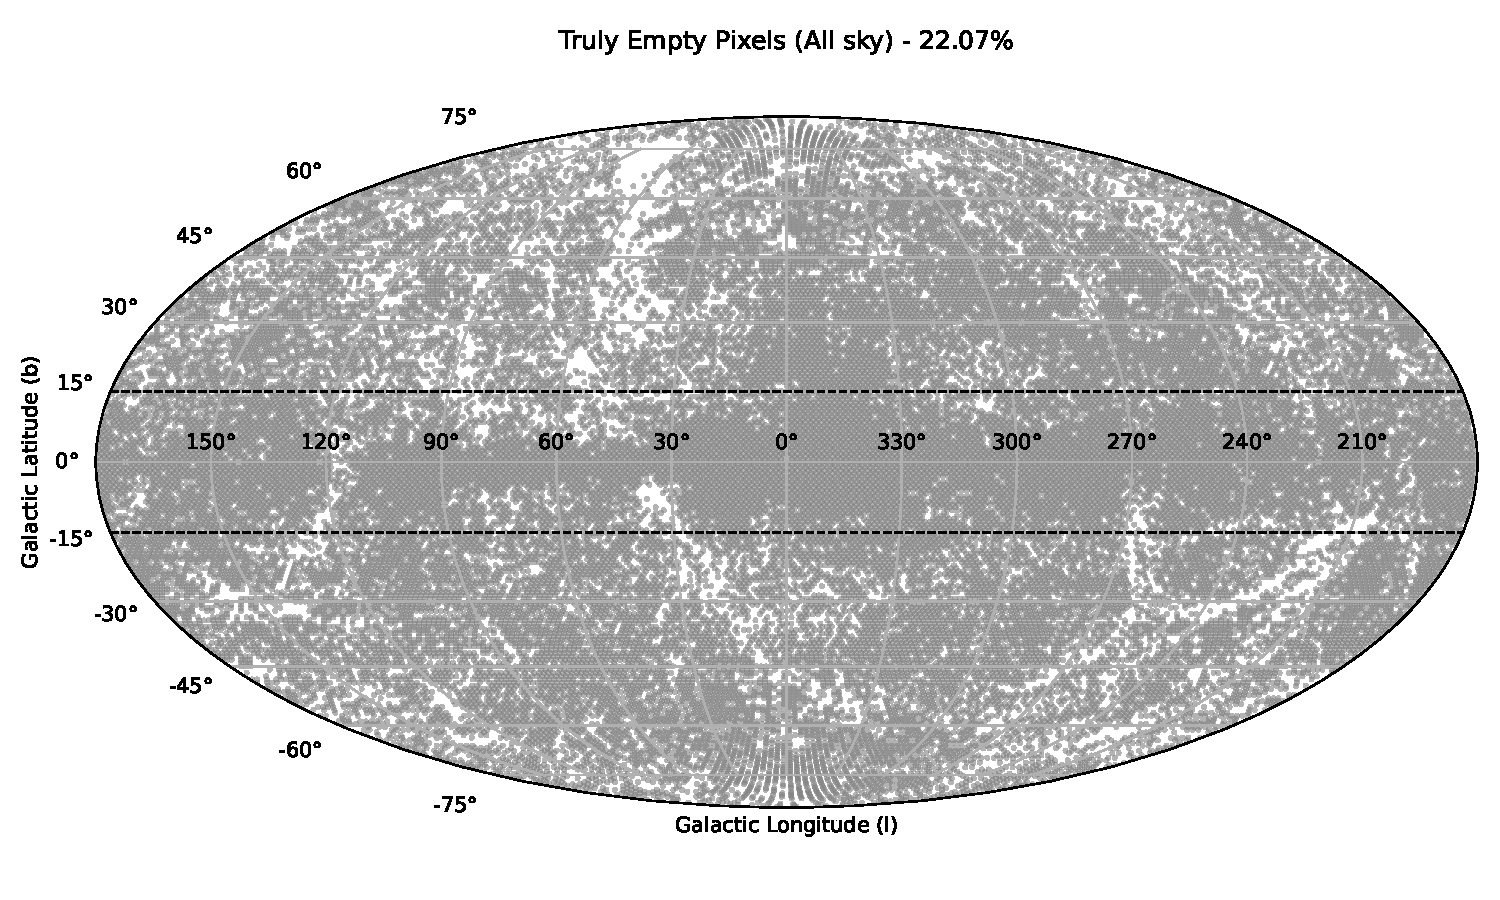
\includegraphics[width=\textwidth]{images/truly_empty_pixels.pdf}
    \end{center}
    \caption{Visual representation of the regions of the sky not covered by any of the 53,255 galaxies in the GWGC, plotted in galactic coordinates using \textbf{healpy}, a Python package that handles pixelated data on the sphere based on the Hierarchical Equal Area isoLatitude Pixelization (\underline{\textbf{\href{https://sourceforge.net/projects/healpix/}{HEALPix}}}). 
    This library allows the user to choose the number of pixels, and thus their size, through a power-of-2 parameter in the \textit{nside2npix} function: the larger the parameter, the smaller the pixel and the bigger their number. 
    The gray dots in the figure represent the empty sky pixels, while the white areas correspond to pixels containing at least one galaxy.
    The central band, where the Milky Way lies, appears significantly emptier than the rest of the sky; this is the so called Zone Of Avoidance (ZOA).
    To estimate the ZOA, we calculated the percentage of empty pixels in the band $|b| \leq 15^\circ$ in Galactic latitude.
    Choosing the parameter to be too small, the produced pixels would be too large, and the empty area would be underestimated.
    Larger values would make the estimation only more precise, and by selecting parameters starting from $2^6=64$, it's possible to estimate roughly $\sim20\%$–$25\%$ of empty sky, fully consistent with the value reported in~\cite{Kraan-Korteweg}.
    The $22.07\%$ estimation in the title is found using $64$ as parameter value.
    }\label{fig: ZOA in galactic coordinates}
\end{figure}
To quantify its extent, we used a Python package that handles pixelated data on the sphere based on the Hierarchical Equal Area isoLatitude Pixelization, \underline{\textbf{\href{https://sourceforge.net/projects/healpix/}{HEALPix}}}, called healpy, to divide the sky map into $n_{\rm pix}$ equal-area pixels, and focused on the band $|b| \leq 15^\circ$ in Galactic latitude.
Counting the empty pixels in this band and dividing by $n_{\rm pix}$ gives an estimated ZOA coverage of $\sim20\%$–$25\%$ of the sky, depending on the chosen pixel resolution.
This estimate is fully consistent with the literature~\cite{Kraan-Korteweg}, so in our analysis we will assume that GWGC effectively covers $\sim80\%$ of the sky.

\subsubsection{Filling the gap}
In order to compensate the missing galaxies, we have made two physically motivated assumptions.
\begin{enumerate}
    \item \textbf{Cosmological Principle}:\\
    The GWGC lists all the observed galaxies within $100Mpc$.
    On such scales, the Universe can be assumed to be statistically \textit{homogeneous} and \textit{isotropic}. 
    This assumption is supported from observations of the \textit{Cosmic Microwave Background} (CMB), where we know that the correlation function of the temperature fluctuations across the sky peaks at scales of $\sim100Mpc$. 
    Under this assumption, the selected galaxies of the GWGC should be statistically representative of the overall population in the same volume, and therefore of the missing galaxies too.
    \item \textbf{Distance}:\\ 
    The angular position is irrelevant in the computation of the gravitational wave signal: only the distance of the source matters.
    Therefore, missing galaxies from the unexplored volume covered by the Milky Way can be statistically represented by the galaxies from our retained sample.
\end{enumerate}
Following these assumptions, we “fill in” the missing fraction of the sky and the dropped entries of the catalog by sampling with replacement from the cleaned GWGC, just like we did to extract an astrophysical population from the fixed one, preserving its parameter distributions.
This ensures that the statistical properties of the synthetic galaxy distribution match those of the observed portion while restoring the full-sky coverage. 
This is shown in a graphical representation of the distributions of distances, blue band magnitudes and T-types, in \textbf{Figure~\ref{fig: distro comparison}}: the distributions have been scaled up without visible changes.
\begin{figure}[h!]
    \begin{center}
        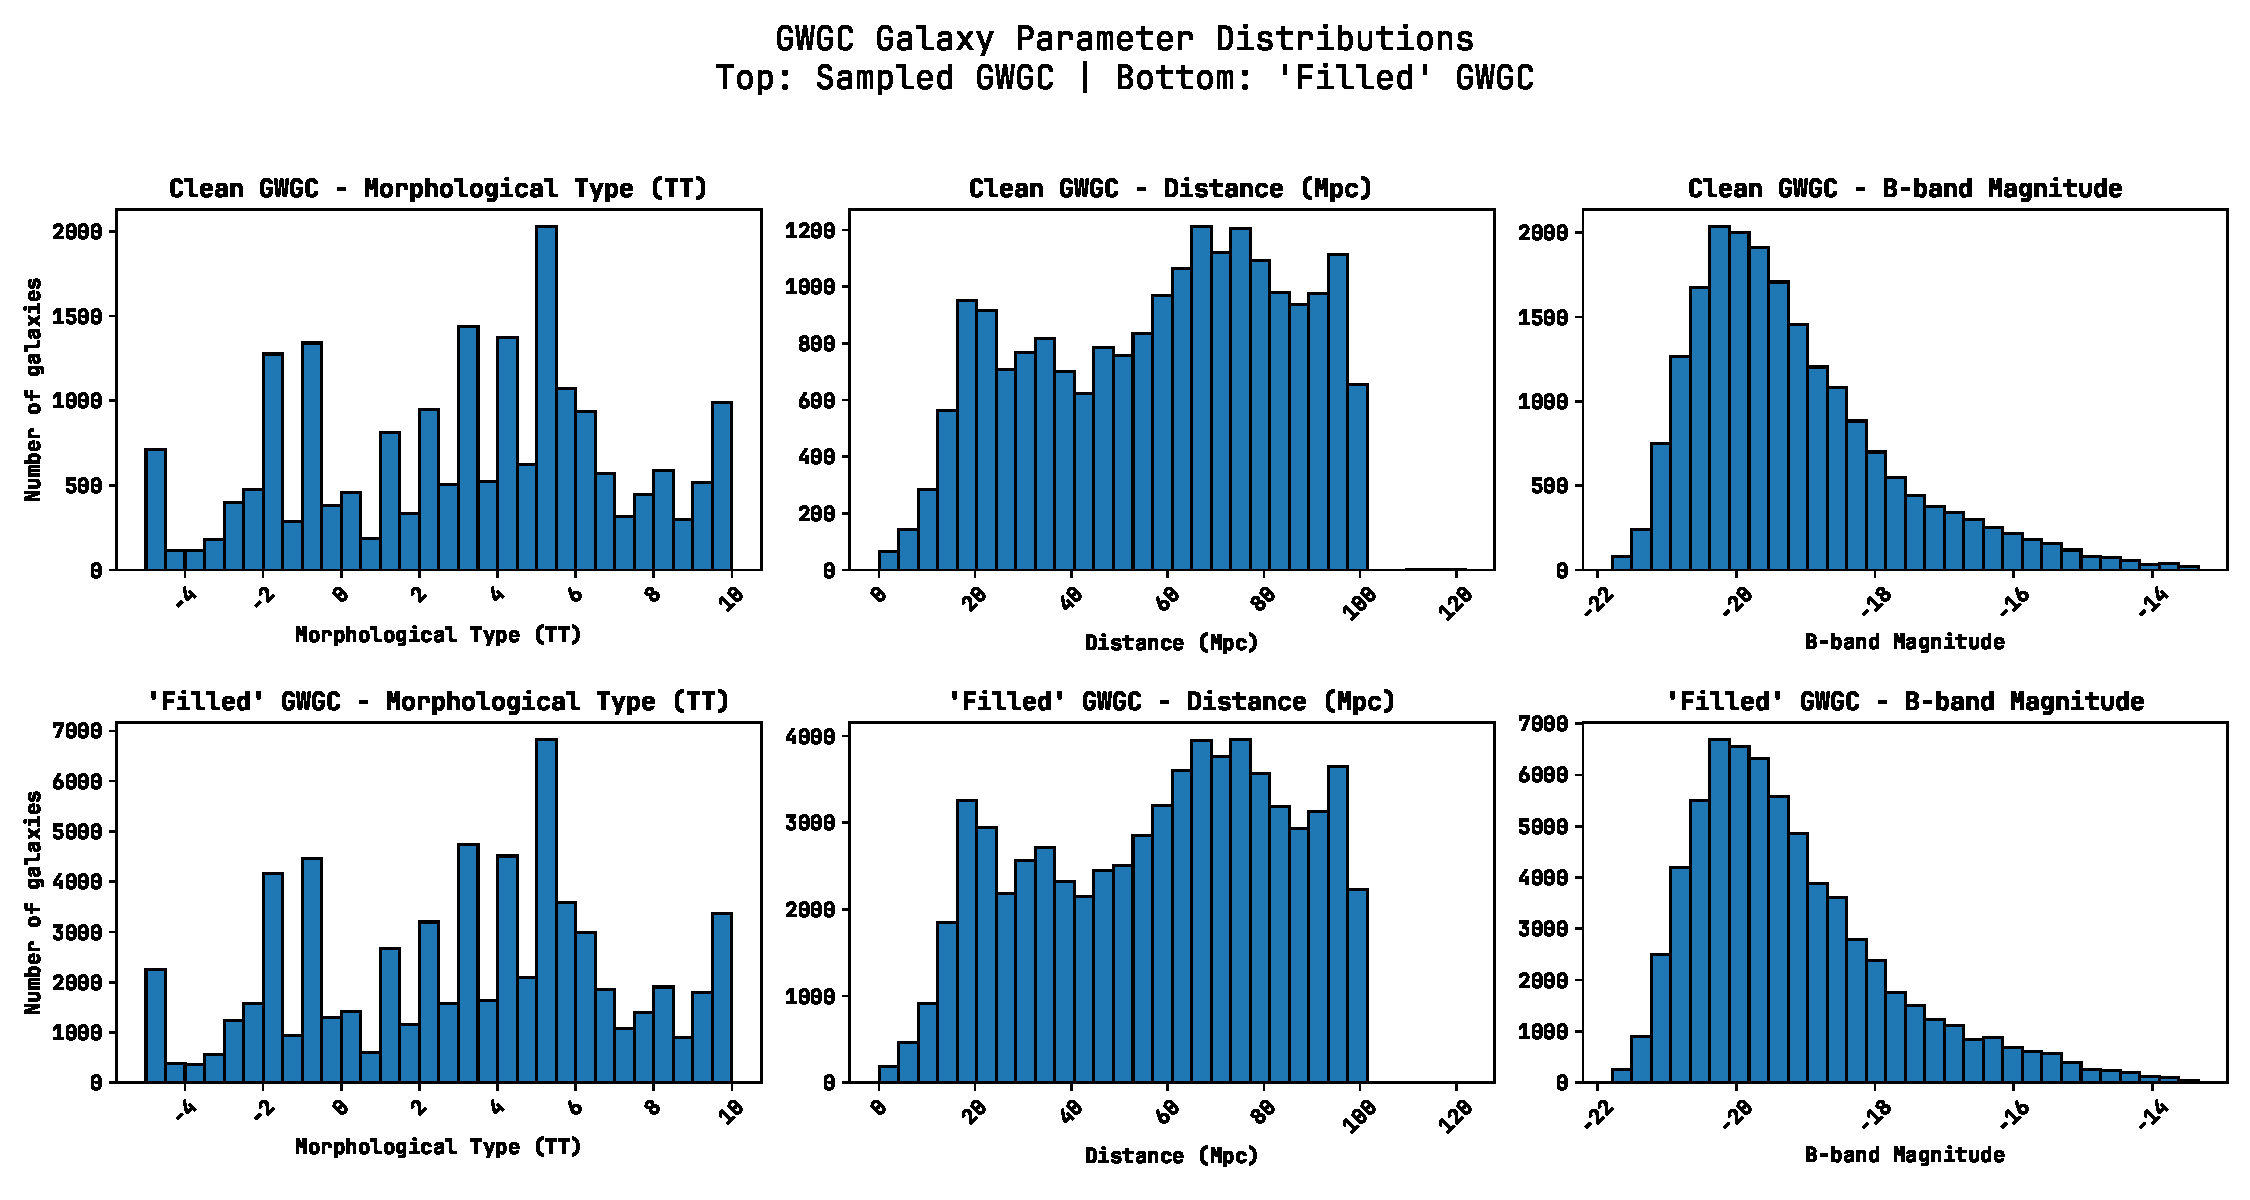
\includegraphics[width=\textwidth]{images/distro_comparison.pdf}
    \end{center}
    \caption{Distributions of T-type, distance and B-band magnitude of the galaxies in the \textbf{Gravitational Wave Galaxy Catalog} (\textbf{GWGC}) before and after compensating for the lack of galaxies due to the catalog's incompleteness and the \textbf{Zone Of Avoidance} (\textbf{ZOA}). 
    The three graphs \textit{above} show the mentioned distributions for the $20,246$ galaxies of the original GWGC after we dropped those missing the key parameters we needed; the three graphs \textit{below} show the same distributions for the $66,568$ galaxies we are left with after taking into account both the catalog's incompleteness and the ZOA using a sampling with replacement method.
    The parameters distributions appear to be indistinguishable in shape: the scaling up in size left the properties of the catalog unchanged.
    }\label{fig: distro comparison}
\end{figure}
\\
The total number of galaxies that we have after taking into consideration both the dropped incomplete entries of the original GWGC and the galaxies covered by the ZOA, has grown to $66,568$.


\subsection{The final fixed populations}
As we already discussed, the metallicity of a galaxy has a great impact on the stellar evolution and, thus, gravitational wave signal.
This, plus the fact that metallicity is also closely linked to the galaxy types, led us to choose it as characterizing parameter for the fixed populations that we will generate to represent the galaxy in the catalog.
In particular, we the final catalog covers a range from a minimum of $ Z= 0.00748$ to a maximum of $Z= 0.03948$.
We decided to group all the values in between in ten equally wide bins, represented in \textbf{Figure~\ref{fig: Z distribution of final catalog}}.
\begin{figure}[h!]
    \begin{center}
        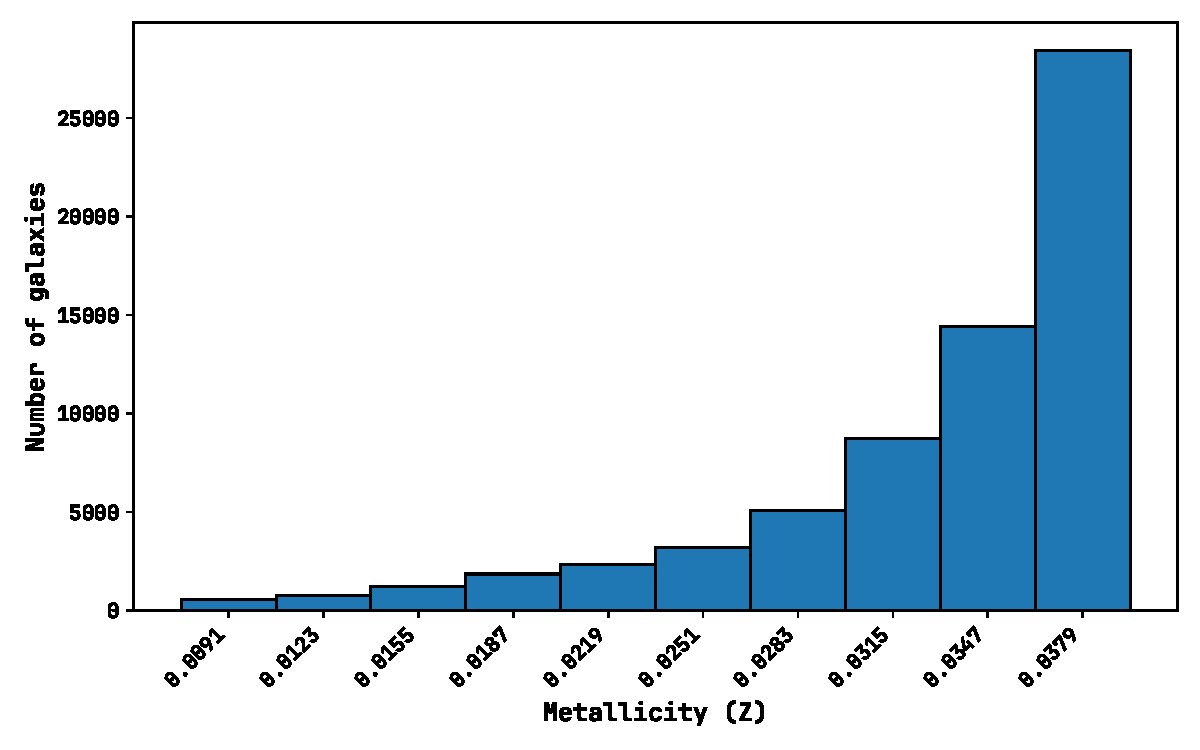
\includegraphics[width=\textwidth]{images/z_distro_gwgc_completed_ZOA.pdf}
    \end{center}
    \caption{Metallicity distribution of the final galaxy catalog. 
    The metallicity of the galaxieshas been shown to correlate with their morphological type~\cite{Faber&Gallagher}.
    Therefore, the entries of our final catalog can be grouped into 10 bins, each associated to a metallicity value (the middle value of the corresponding bin, shown in the $x$-axis label of the graph), and a corresponding fixed population.
    }\label{fig: Z distribution of final catalog}
\end{figure}\\
Each one of the bins center values, shown in the $x$ label, is linked to a different synthetic fixed population generated with COSMIC.
The simulations were done generating the fixed populations "\textit{\href{https://cosmic-popsynth.github.io/docs/stable/pages/fixedpop.html}{the cosmic way}}", via terminal, specifying $Nstep = 5000$ and $Niter=1000000000$ and kstar values $10$, $11$ and $12$, corresponding to He, CO, and Ne white dwarfs\footnote{All the kstar values and the corresponding astrophysical objects are shown in \textbf{Table~\ref{tab: kstar values}}, in the \textbf{Appendix}.}, assuming the sun's metallicity to be $Z_\odot = 0.0134$ and leaving all the remaining COSMIC's specifiable parameters unchanged from the default values.


\section{The Signal Computation}
Generating the DWDs using COSMIC gives us the possibility to calculate the gravitational wave contribution of each one of them, assuming their distance to be the same as the hosting galaxy's one, provided from the galaxy catalog, and with an extreme precision in frequency.
Before scaling up the fixed population, and calculating each binary's gravitational wave signal, and confronting it with LISA's sensitivity curve, we must then consider LISA's limited \textit{frequency resolution}, and understand how to process the signals of indistinguishable sources.
This will allow us to finally find if LISA's curve will be affected by the unresolved extragalactic DWDs gravitational wave confusion foreground.

\subsection{LISA's frequency resolution}
The duration of LISA’s mission directly impacts its frequency resolution: the longer the observation time, the finer the frequency bins it can resolve.
In this work, we assume an observation time of: 
\[
    T_{obs}=4yr=126,144,000s
\]
which corresponds to a minimum frequency resolution of
\begin{equation}
    \delta\nu_{LISA,\min}\approx \frac{1}{T_{obs}}\sim 8\times 10^{-9}Hz.
    \label{eq: LISA frequency resolution}
\end{equation}
This fundamental limit comes from the Fourier transform properties, and determines the smallest frequency interval over which the signals can be resolved.
Although this is a very fine resolution, the precision of the orbital period in the simulated binary systems, and thus the frequency resolution on their gravitational signal, is actually much bigger, since these values come from a simulation rather than from real observations.
For this reason, when computing the gravitational wave signals of our simulated binaries, we must take into account the fact that LISA will not be able to distinguish sources within the same frequency bin.
To model this, we group the resulting gravitational wave signals in bins of size $\delta\nu_{LISA,\min}$, and sum all the signals that fall within each bin, as we will now explain.

\subsubsection{Signals summation}
To accurately represent the frequency resolution limit imposed by LISA's observation time, we have to sum all the signals within the same frequency bin. 
In principle, over the observation time $T_{obs}$, the orbital parameters of the sources may slowly evolve, causing a drift in the gravitational wave frequency. 
Integrating the resulting signal during this period is no easy task.
However, for the slowly evolving white dwarf binaries we are considering, the change in such short time-frames is negligible, so we can treat their signals as effectively monochromatic within the observation window. 
Thus, we can define a commonly used variable to simplify our job, which is called  \textbf{Amplitude Spectral Density} (\textbf{ASD}):
\begin{equation}
    ASD = h\sqrt{T_{obs}},
    \label{eq: ASD definition}
\end{equation}
where $h$ is the gravitational wave strain of the binary, computed in~\eqref{eq: the strain we use}, and $T_{obs}$ is the mission duration for LISA.
This quantity represents the characteristic strain amplitude of the gravitational wave signal per square root of frequency, scaled by the observation time, and its very convenient for comparing the signals in frequency space.
Correspondingly, we can define the \textbf{Power Spectral Density} (\textbf{PSD}) as the square of the ASD
\begin{equation}
    PSD = ASD^2,
    \label{eq: PSD definition}
\end{equation}
which properly represents the signal power per frequency unit.
Since power contributions from independent sources add linearly, the total PSD in a given frequency bin is simply found by summing the power of all the sources within it:
\begin{equation}
    PSD_{tot,bin_1} = PSD_{1,bin_1} + PSD_{2,bin_1} + \dots
    \label{eq: total PSD}
\end{equation}
This way, we effectively accounted for LISA's frequency resolution limit.
The reason for introducing this quantities is that gravitational waves from different binaries are uncorrelated, so their strains add incoherently. 
This means we cannot simply sum the strain amplitudes directly.
Instead, the PSD provides a way to combine signals that ensures a correct representation of the combined gravitational wave background.

\subsection{The pipeline}
In order to compute the total extragalactic DWDs gravitational background, we must apply an iterative process to each galaxy in the final catalog, which consists of the following steps:
\begin{itemize}
    \item Compute the right $N_{astro}$ using the~\eqref{eq: scale by mass}
    \item Scale the fixed population accordingly with a sampling with replacement method, creating the full-size galaxy simulation.
    \vspace{1.5mm}\\
    At this point for each binary system in this astrophysical population we:
    \begin{itemize}
        \item Compute the gravitational wave signal using~\eqref{eq: the strain we use}\footnote{Note here that all the binaries within the same galaxy are given the same distance from us. This approximation is considered to be valid since the distance of the galaxy is much much bigger the its size, and thus the maximum possible distance between two binaries within the same galaxy.} and the corresponding $PSD$ using~\eqref{eq: ASD definition} and~\eqref{eq: PSD definition};
        \item Sum the total PSD of the binaries whose frequencies fall within the same LISA's frequency bin, using~\eqref{eq: total PSD};
        \item Plot the total binned signals on LISA's curve.
    \end{itemize}
\end{itemize}
\subsubsection{LISA's sensitivity curve}
The LISA curve is constantly updated when new gravitational wave components that can affect it are found, meaning that there are many different versions around.
The one we chose to use is the widely used version presented in~\cite{Robson_2019}, which is written as:
\begin{equation}
    S_n = \frac{10}{3L^2} \left( P_{OMS}(f) + \frac{4P_{acc}(f)}{(2\pi f)^4} \right)\left( 1 + \frac{6}{10}\left(\frac{f}{f_*}\right)^2 \right) + S_c(f),
    \notag
    %\label{eq: LISA sensitivity curve by Robson}
\end{equation}
where $L=2.5 Gm$ is the LISA arm length, $f_*=19.09mHz$ and $P_{OMS}(f)$, $P_{acc}(f)$ and $S_c(f)$ are the expressions for the single-link optical metrology noise, the single test mass acceleration noise and the total Michaelson-style LISA data channel. 
The equations for these factors, as well as more detail on the curve that we chose, can be found in the article.


\section{Discussion}

Doing this, the spectral distribution of the final resulting signal is plotted over the LISA's sensitivity curve\footnote{This particular curve is presented in~\cite{Robson_2019}.} in \textbf{Figure~\ref{fig: Final results plot}}
\begin{figure}[hb!]
    \begin{center}
        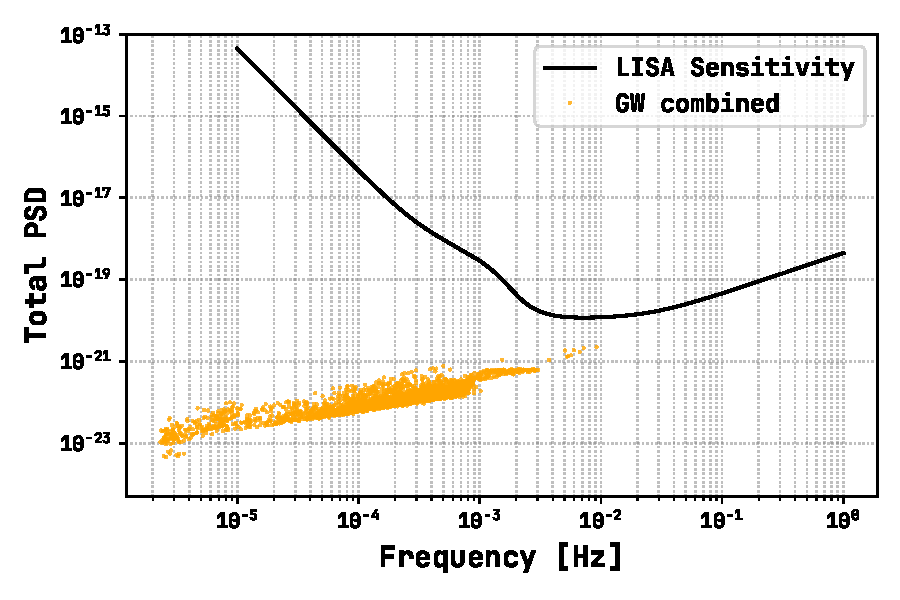
\includegraphics[width=\textwidth]{images/Final_results_plot.pdf}
    \end{center}
    \caption{Total gravitational wave signal of the simulated Double White Dwarfs (DWDs) hosted by the $66,568$ galaxies of the final catalog, binned in $\sim 8\times10^{-9}Hz$ large frequency bins, representing LISA's spectral resolution. 
    Every orange dot represents the signal of a frequency bin, calculated by summing the Power Spectral Density (PSD) of every galaxy that it contained, using~\eqref{eq: total PSD}. 
    The dots are plotted on LISA's sensitivity curve, as found in~\cite{Robson_2019}, and appear to be about one order of magnitude below the minimum threshold of this curve.
    This results suggest that we should not expect LISA to be able to detect the unresolved extragalactic DWDs confusion foreground, at least under the assumptions and approximations adopted in this work.}\label{fig: Final results plot}
\end{figure}
Every orange dot in this graph represents a frequency bin, whose width is given by~\eqref{eq: LISA frequency resolution}, where the gravitational wave signal of all the binaries within it has been summed using~\eqref{eq: total PSD}.
The resulting calculated signal appears to be about one order of magnitude smaller than the minimum detectable strain for LISA across the whole band.  
This indicates that, luckily, the stochastic contribution from unresolved extragalactic DWDs will not have a measurable impact on LISA’s sensitivity curve, at least under the assumptions of our population model and scaling relations. 

\paragraph{Distribution of the sources}
The simulated extragalactic binaries foreground populates primarily the low-frequency range ($f \lesssim 2\,\mathrm{mHz}$), with the number of systems per frequency bin increasing steeply at higher frequencies. 
This is evident for at least two reasons:
\begin{enumerate}
    \item The orange dots seem to be more sparse at lower frequencies, and increasingly densely packed towards higher frequencies, showing that more empty bins appear to be at the lower end of the spectrum, and the more populated ones at the higher end;
    \item The sources appear to lay on a slope, with the PSD values steadily increasing with the frequency, showing that at higher frequencies, the occupied frequency bins tend to be more and more populated, and therefore the total PSD they contain higher and higher in magnitude.
\end{enumerate}
A possible physical explanation for this phenomenon is that the time evolution of the orbital parameters is initially very slow, allowing the orbital frequencies to distribute over a wider range of bins.
As the binary systems evolve they get more compact, and the parameters change more rapidly, increasing the likelihood that the systems occupy very close frequency bins.
Moreover, the spectral shape of the resulting background is positioned at frequencies that are similar to the expected Galactic foreground ones (corresponding to the slight bump at the left of the lowest point in the graph. 
This is better shown in \textbf{Figure~\ref{fig: LISA sens curve with noises}}), but with a significantly lower amplitude due to the much larger average distances.
Indeed, as shown in~\eqref{eq: the strain we use}, the gravitational wave amplitude scales inversely with the distance from the source, so even relatively nearby galaxies contribute far less per binary than the Milky Way population. 
The total number of galaxies in the local Universe, even if large, is not sufficient to compensate for this distance-induced amplitude suppression in the LISA band.


\subsection{Stability of the results}
The simulated gravitational wave signal, represented by the orange dots, would be detectable by LISA if it fell above the LISA curve, meaning that the total PSD in a certain frequency bin is higher than the minimum threshold of LISA's sensitivity.
Therefore, the dots can get close to, or above the sensitivity curve either by containing extremely close and strong sources, by containing the contribution of many farther, and fainter sources, or a combination of both.
In principle, the results we presented could depend on the assumptions we made, and the methods we used.
In particular, for what we have just said, the most important steps we took in this regard are and the calculation of the signal, and the representation the sources.

\subsubsection{The sources}
The results could be affected by the way we represented the sources, via GWGC.
Indeed, this is the input we give our pipeline to produce, as an output, what should be the total gravitational wave confusion foreground from all the unresolved DWDs in the local universe.
For example, if we only used the GWGC catalog after dropping the incomplete voices, and without considering the zone of avoidance, the total gravitational wave signal produced by the remaining $20,246$ galaxies would be as represented in \textbf{Figure~\ref{fig: total signal plot with incomplete catalog}}.
\begin{figure}
    \begin{center}
        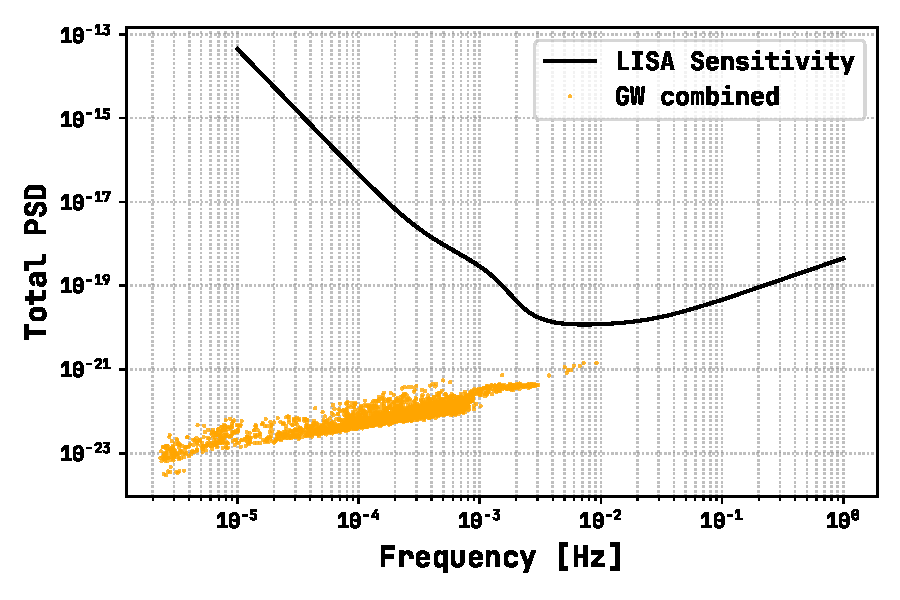
\includegraphics[width=\textwidth]{images/Final_results__incomplete_GWGC_plot.pdf}
    \end{center}
    \caption{Total gravitational wave signal of the simulated Double White Dwarfs (DWDs) hosted by the $20,246$ galaxies of the GWGC after dropping the galaxies with incomplete information, and without considering the zone of avoidance. 
    The signal is binned in $\sim 8\times10^{-9}Hz$ large frequency bins, representing LISA's spectral resolution. 
    Every orange dot represents the signal of a frequency bin, calculated by summing the Power Spectral Density (PSD) of every galaxy that it contained, using~\eqref{eq: total PSD}. 
    The dots are plotted on LISA's sensitivity curve, as found in~\cite{Robson_2019}, and appear to be about one order of magnitude below the minimum threshold of this curve.
    This results, if compared with the ones showed in \textbf{Figure~\ref{fig: Final results plot}}, show that the effect of not taking into account the missing galaxies is very small, barely noticeable. 
    }\label{fig: total signal plot with incomplete catalog}
\end{figure}
Although a slight difference in height with the results obtained for all the $66,568$ galaxies presented in \textbf{Figure~\ref{fig: Final results plot}} is noticeable, it is important to note that it is caused by considering less then a third of the sources.
Therefore, even if it is possible to consider different and more complete catalogs, and the zone of avoidance could be estimated with better precision, the results we found do not depend significantly on this.
In addition to this, the single DWDs were simulated using COSMIC, which represent and arbitrary choice between a number of different population synthesis codes: this might produce different sources parameter distributions, and could be an interesting extension of the present work.

\subsubsection{The signal}
The main assumptions we made to obtain the results are surely how we calculated the gravitational wave characteristic strain, and the way we integrate the signal coming from unresolved sources within the same frequency bin.
The gravitational wave signal calculated in~\eqref{eq: the strain we use} is the standard characteristic strain predicted from the General Relativity for an inspiraling binary system, and is therefore the most precise way to represent the DWDs signal.
Furthermore, the use of Amplitude Spectral Density (ASD) and Power Spectral Density (PSD) is unavoidable, since it is the only way to confront signals that LISA could not resolve in frequency with its sensitivity curve.
Interestingly, assuming a longer observational time would guarantee LISA a better frequency resolution, and each frequency bin would appear to be less populated.
Since, as we said, less populated bins generally contain lower total PSD, the better the LISA's frequency resolution, the lower the sensitivity to the noise that the unresolved sources produce, and therefore the lower LISA's sensitivity curve needs to be to detect it.
In any case, the methods we used guarantee a pretty stable and reproducible output, given the same input.


